\documentclass[a4paper,12pt]{article} % Changer la taille de police c'est ici

\usepackage{framed} % Marges
\usepackage[utf8]{inputenc} %francais
\usepackage[T1]{fontenc} %francais
\usepackage[french]{babel}  %francais
\usepackage{lmodern} % Pour changer le pack de police
\usepackage{makeidx} % Index
\usepackage{graphicx} % Figures
\usepackage{wrapfig} % Figures
\usepackage{amsmath} % Maths
\usepackage{amssymb} % symboles ?
\usepackage{bclogo} % ?????
\usepackage{hyperref}
\usepackage{stmaryrd}
\usepackage[top=2cm, bottom=2cm, left=2cm, right=2cm]{geometry} %Marges

\title{Rapport Interpolaspline}
\author{Interpolaspline}
\date{Avril 2020}

\begin{document}

\maketitle

\section{Introduction}

\section{Théorie sur l'interpolation}

\subsection{Définitions}

Une spline naturelle cubique $C^{2}$ est une fonction définie par morceaux par des polynômes cubiques, dont la dérivée seconde est continue et dont les dérivées secondes aux extrémités de l'intervalle de définition sont nulles. 

Une spline de lissage est une fonctions qui minimise une certaine quantité liée à la différence entre la courbe et les données mesurées. L'identification des valeurs aberrantes sera implémentée pour ensuite les supprimer avant de créer la spline, ou pour leur attribuer un poids faible lors de la minimisation de la quantité.

\section{Reprise des Bases}

\subsection{Objectif}

Le but, avant de commencer le vif du projet, était de reprendre les programmes écrits pendant les cours d'algèbre linéaire pour le graphique et la CAO. Ces programmes sont adaptés à des énoncés de travaux pratique, il faut donc les reprendre pour les compléter et les adapter à nos besoins.

Ces programmes seront la base du projet.

\subsection{Splines naturelles}

Dans cette partie, il est traité de l'interpolation par spline naturelle cubique $C^{2}$.

Le programme adapté possède trois principales fonctionnalités. Toutes s'appuient sur la lecture d'un fichier et créent une courbe (paramétrique ou non) interpolant les données.
Le choix de l'ordre des points est donné à l'utilisateur sous la forme de trois choix : 


\begin{itemize}
    \item[•] Traitement des données "telles quelles". Les données sont traitées dans l'ordre dans lesquelles elles ont été fournies, sous forme de courbe paramétrique.
    \item[•] Traitement des données selon la première coordonnée. Les données sont triées par ordre croissant selon la première coordonnée. Cela permet d'éviter d'avoir une courbe paramétrique qui reviendrait sur ses pas. La courbe obtenue est une fonction de $\mathbf{R}$ dans $\mathbf{R}$.
    \item[•] Traitement des données selon la deuxième coordonnée. Cela correspond à la même manipulation que précédemment, mais selon la deuxième coordonnée.
\end{itemize}





\begin{figure}[h]
\begin{center}
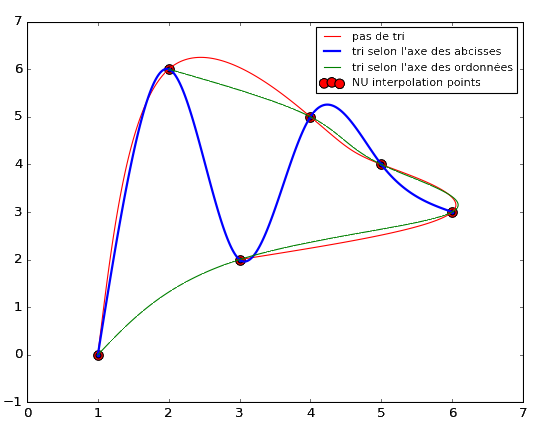
\includegraphics[width=8cm]{tache0.png} 
\end{center}
\caption{Exemple des trois modes de traitements des données}
\end{figure}


\end{document}
